% !TeX root = ../thuthesis-example.tex

\chapter{系统实现:大数据机器学习研发管理系统Anylearn}

Anylearn是一款大数据机器学习研发管理系统,支持数据集、算法族、模型库等资产管理,支持机器学习研发过程管理、知识沉淀、模型迁移,满足团队资源统筹利用、团队高效协作等人工智能工程化需求。

Anylearn包括:
\begin{itemize}
  \item Anylearn云环境,即Anylearn长活系统线上环境(https://anylearn.nelbds.cn/);
  \item Anylearn交互网页,即Anylearn云环境的Web页面;
  \item Anylearn客户端SDK(https://pypi.org/project/anylearn/)。
\end{itemize}

Anylearn交互网页的主要模块包括:训练项目、数据集、算法族、模型库、镜像中心、计算资源概况以及用户中心等。


\section{使用场景}

\subsection{场景一:将本地机器学习项目适配至Anylearn云环境}

用户在本地(PC、开发服务器等自有环境)已开展机器学习项目的研发,已经明确了要使用的数据集、算法、预训练模型。算法经调试,已成功在本地运行了小规模训练。
用户希望将此机器学习项目适配到Anylearn云环境,使用更多算力和研发管理功能进行更大规模的训练和验证。

具体步骤如图\ref{fig:scenario1}所示。

\begin{figure}
  \centering
  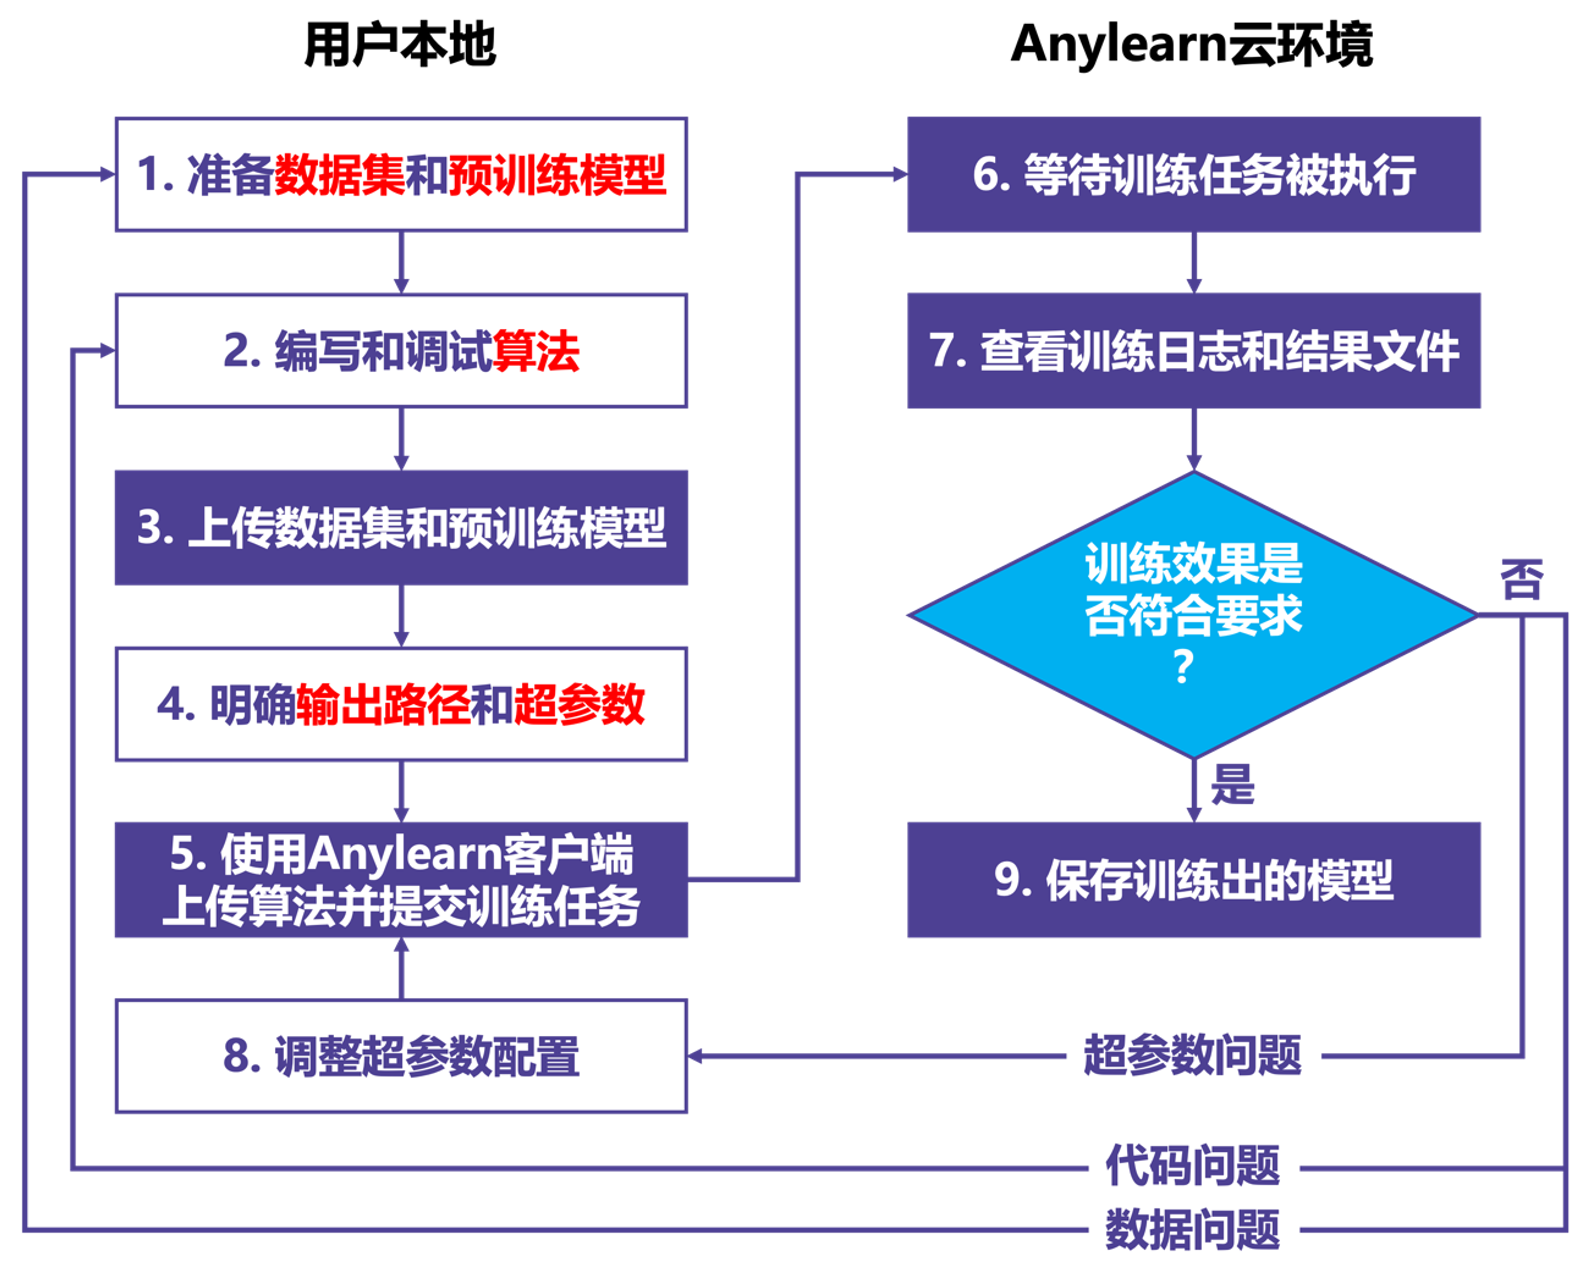
\includegraphics[width=0.8\linewidth]{anylearn-scenario1.png}
  \caption{Anylearn使用场景一:本地项目适配至云环境}
  \label{fig:scenario1}
\end{figure}

(1)用户根据机器学习项目需求,在本地已准备好数据集和预训练模型。
根据机器学习任务的不同,可能会使用一个或多个数据集和预训练模型(例如:域适应迁移学习),也可能不需要数据集和模型。

(2)用户在本地已编写并调试好机器学习算法,已在本地使用上述数据集和预训练模型初步跑通训练和验证。

(3)用户前往Anylearn交互网页并注册账户。
然后,用户通过Anylearn交互网页将步骤1中的数据集和预训练模型分别上传至Anylearn云环境。
当数据集或预训练模型的规模较大时(依据经验,超过500MB即为大),通过Anylearn交互网页上传效率较低,应当联系Anylearn系统管理员通过其他方式上传。
需要注意的是,由于网络条件有限,在Anylearn云环境中执行训练时从外网下载数据集和模型通常非常缓慢,使用torchvision、huggingface等库进行自动下载的数据集和模型需要提前上传到Anylearn云环境。

(4)用户需梳理并明确机器学习算法的输出路径和超参数。
输出可能包括:模型检查点文件(checkpoints)、最终模型参数文件(weights)、TensorBoard日志文件、模型验证效果文件等等。
Anylearn云环境中要求这些输出均需要写入到一个统一的路径下,该路径应当是以算法目录下的一个子目录(例如:假设用户本地的算法存放在/workspace/myuser/myalgo下,本步骤中涉及的输出可以写入./results目录,即绝对路径/workspace/myuser/myalgo/results,但不可写入算法目录以外的/data/results路径下)。

(5)用户在本地安装Anylearn客户端SDK。
用户可能需要修改步骤(2)中的本地算法代码。
用户在本地编写一个Python脚本,调用Anylearn客户端库(SDK),将本地算法上传至Anylearn云环境,并向Anylearn云环境提交一个训练任务。

(6)用户前往Anylearn交互网页,查看上述提交的训练任务的状态。
由于计算资源有限,提交的训练任务可能无法马上执行,需排队等待资源释放。

(7)当训练任务开始执行后,用户在Anylearn交互网页中查看训练任务的日志、系统监控等信息,判断训练执行情况以及训练出的模型的效果。

(8)当用户发现训练有问题时:
\begin{enumerate}
  \item 当训练超参数存在问题时,用户在本地算法或步骤5中编写的本地Python脚本中修改超参数配置,重新执行本地Python脚本以上传修改后的算法并提交一个新的训练任务,即重复步骤(5)及其后续步骤;
  \item 当训练代码(例如:数据加载方式、模型架构、优化器使用等等)存在问题时,用户调整本地算法代码,上传修改后的算法并提交一个新的训练任务,即重复步骤(2)及其后续步骤;
  \item 当数据集存在问题时,用户调整数据集或重新准备数据集,并将修改后的数据集当做一个新的数据集上传至Anylearn云环境(已存在的数据集不支持变更文件),即重复步骤(1)及其后续步骤。
\end{enumerate}

(9)当用户认为训练出的模型达到预期效果时,用户在Anylearn交互网页上将训练出的模型参数文件转存至Anylearn云环境的模型库,形成模型资产。

\subsection{场景二:参与Anylearn云环境上已存在的机器学习项目}

机器学习项目组已在Anylearn上开展工作,用户作为新进组的成员,对已经在Anylearn云环境中跑通的算法进行迭代优化。
用户需将项目组先前上传至Anylearn云环境的数据集、预训练模型和算法下载至本地(PC、开发服务器等自有环境),对算法进行调整,再将算法上传回Anylearn云环境并进行训练和验证。

具体步骤如图\ref{fig:scenario2}所示。

\begin{figure}
  \centering
  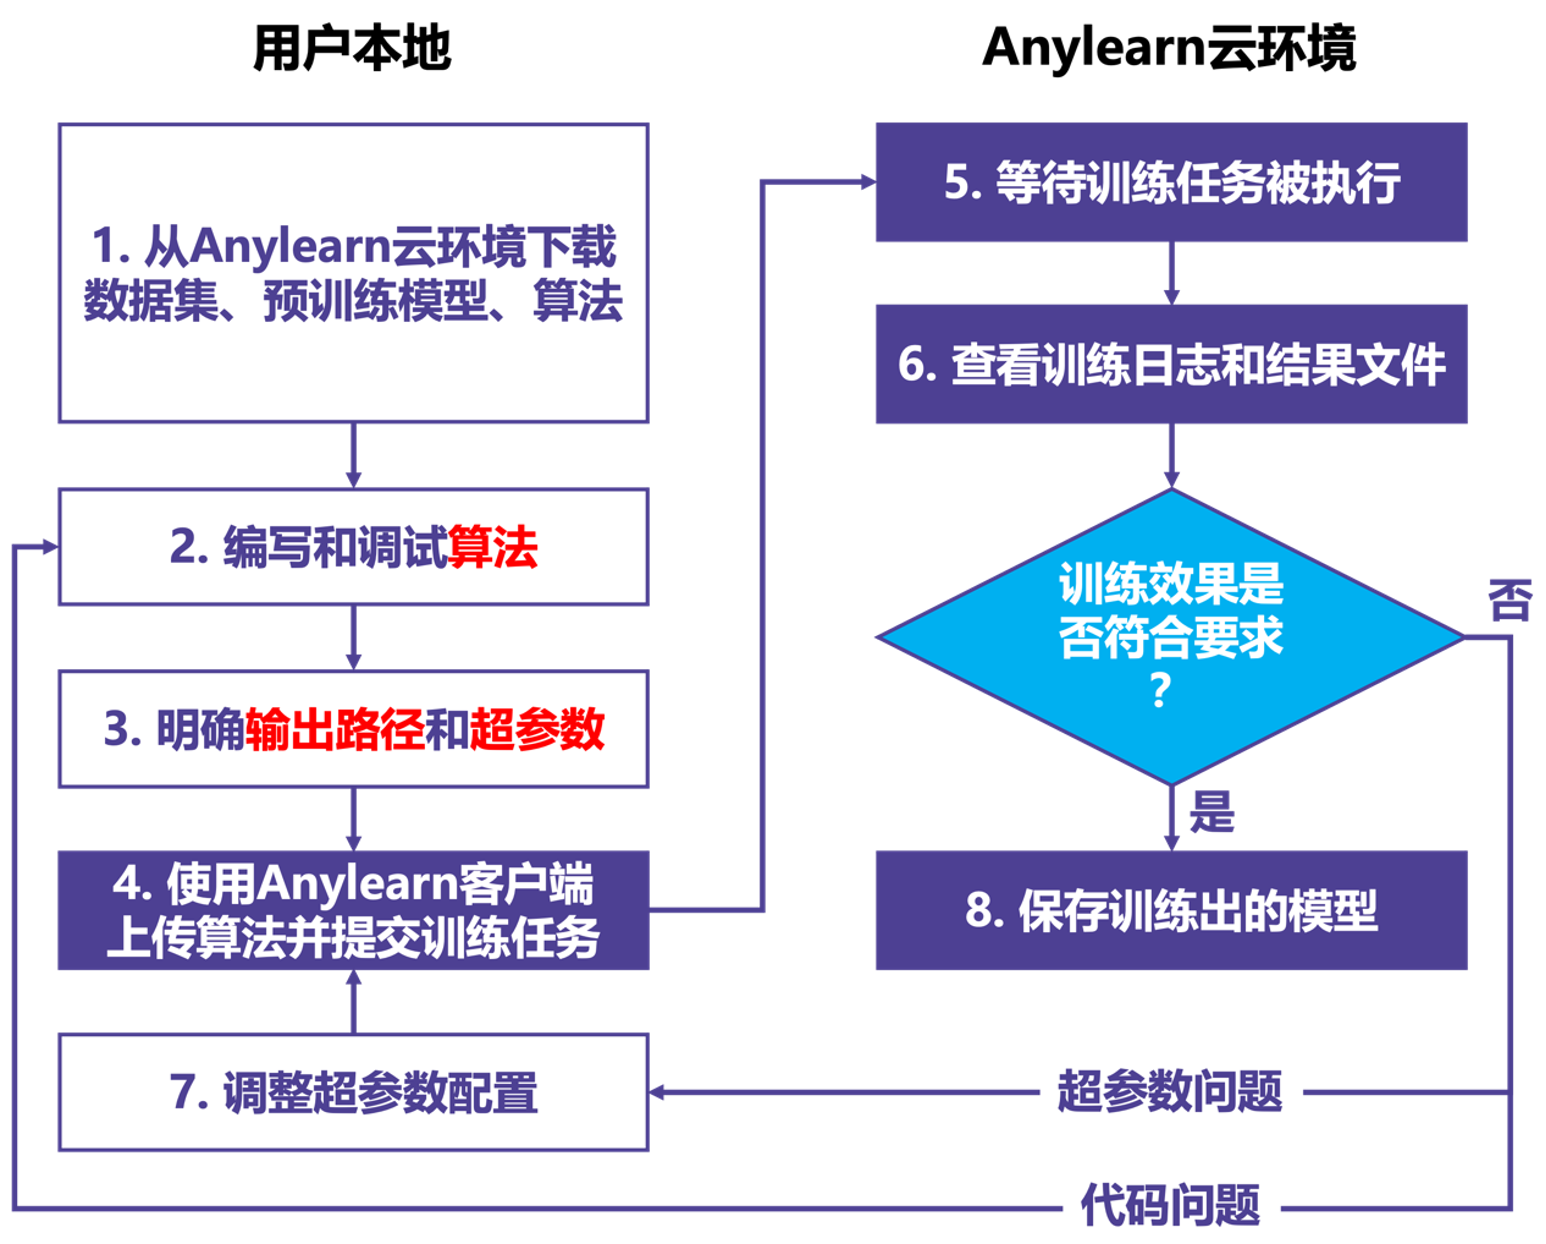
\includegraphics[width=0.8\linewidth]{anylearn-scenario2.png}
  \caption{Anylearn使用场景二:参与云环境中的项目}
  \label{fig:scenario2}
\end{figure}

(1)用户按照项目组要求,通过Anylearn交互网页将Anylearn云环境中的数据集、预训练模型和算法下载至本地。
由于网络条件有限,从Anylearn交互网页上下载较大规模的数据集和模型(依据经验,GB级以上即为大)通常非常缓慢,应当联系Anylearn系统管理员通过其他方式下载。

(2)用户在本地修改算法代码并调试,确保修改后的代码在本地使用上述数据集和预训练模型初步跑通训练和验证。

(3)后续步骤请参考场景一的步骤(4)至(9)。


\section{架构设计}

TBD


\section{功能设计}

TBD


\section{线上环境}

“实践是检验真理的唯一标准”这一理念对于软件尤为重要,敏捷开发方法论中也强调了用户反馈对软件迭代的意义。
为了验证Anylearn的能力并持续打磨其功能性能,2021年7月起,Anylearn在大数据系统软件国家工程研究中心的私有云进行了部署,作为一套公开长活的线上系统对外提供服务,供软件学院、研究中心以及其他相关科研团队使用。

\subsection{集群架构}
Anylearn线上环境中配备了11台高性能GPU服务器,每台服务器配备4张GPU,共计44张,包括24张NVIDIA A100(其中20张为40G显存版,4张为80G显存版)和20张NVIDIA GeForce RTX 3090。
Anylearn依托私有云的网络环境,通过搭建Kubernetes集群池化纳管所有GPU服务器。
Kubernetes集群中使用了私有云的3台虚拟机作为主节点形成控制面,并通过内网负载均衡器与GPU服务器连通,实现了集群的高可用,即任意2个主节点下线均不影响集群任何功能的访问。
集群节点的架构如图\ref{fig:cluster}所示。

\begin{figure}
  \centering
  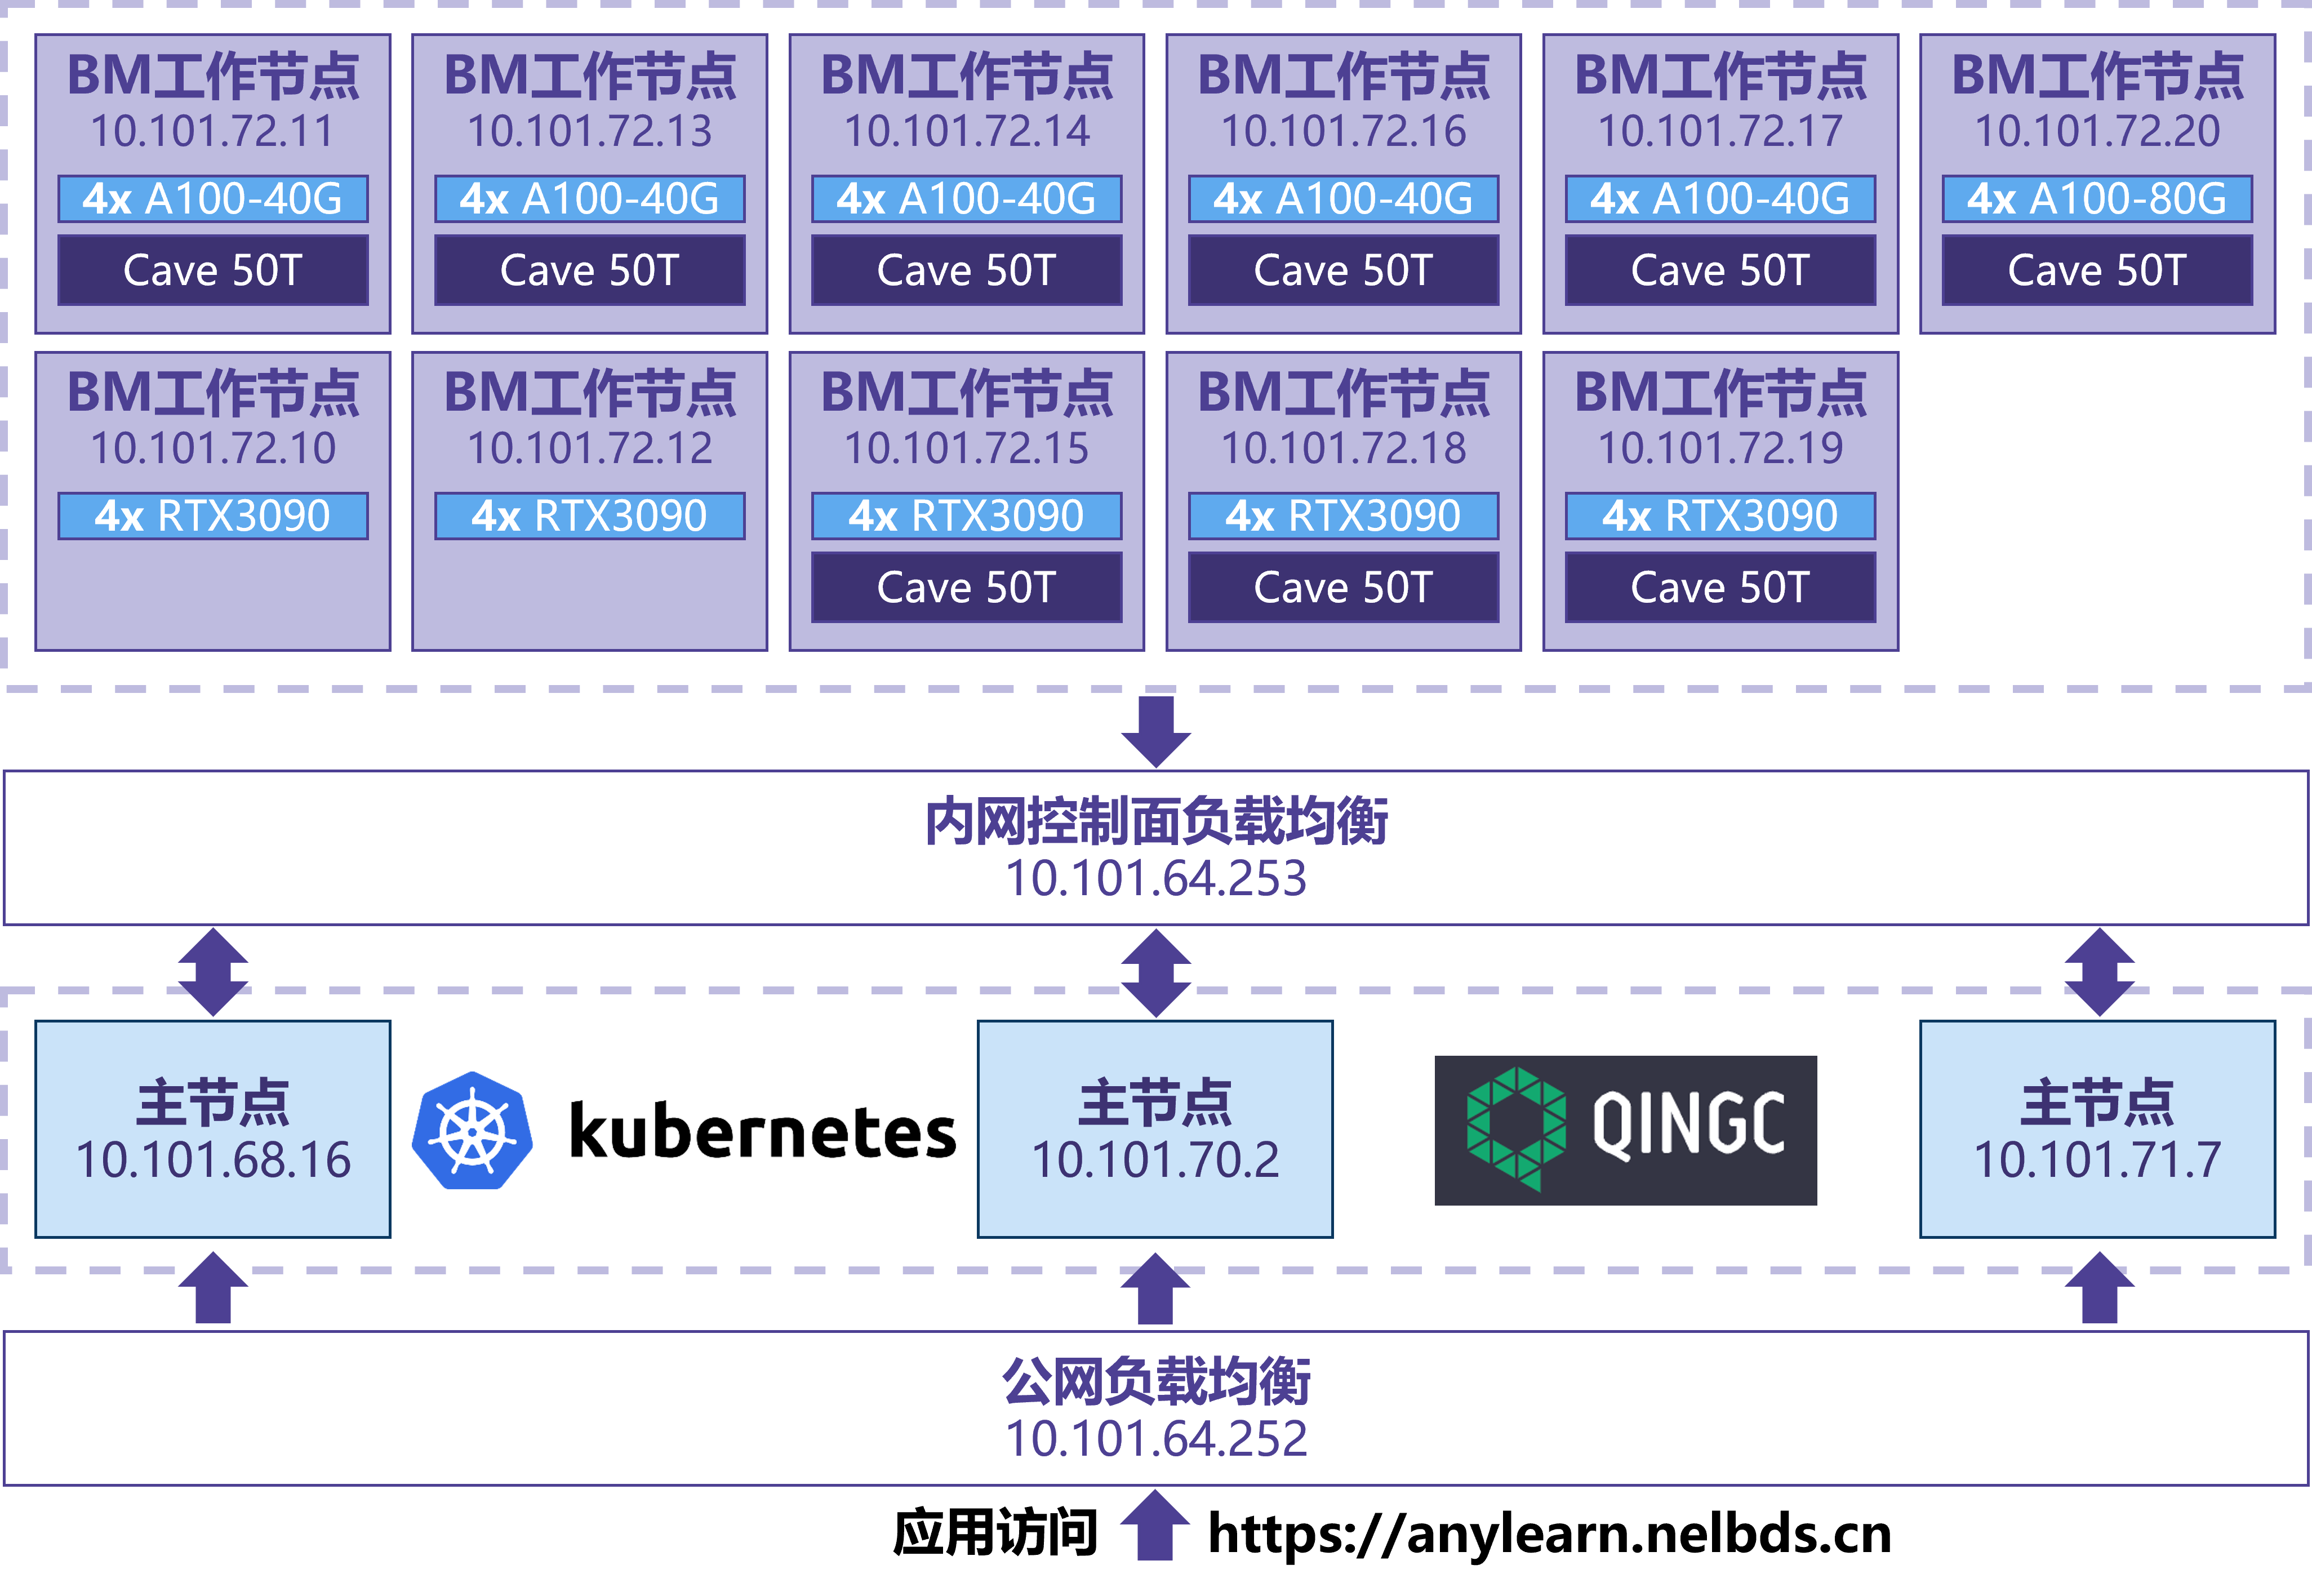
\includegraphics[width=0.98\linewidth]{anylearn-cluster-structure.png}
  \caption{Anylearn线上环境集群架构}
  \label{fig:cluster}
\end{figure}

集群架构经历过7次较大的变动:
(1)2021年7月首次部署时,集群中包含了9台GPU服务器,其中2台未配备GPU,故用作Kubernetes集群控制面的双主节点形成伪高可用架构;
(2)2021年9月,集群中GPU齐备,数量为36张,原用作主节点的2台GPU服务器应当专用于GPU算力负载,不再适合分散其负载能力到控制面,故使用3台私有云虚拟机作为集群主节点,形成真正高可用的集群控制面; 
(3)2022年6月,由于集群证书配置问题导致集群不可用,重新部署了集群并调整了主节点虚拟机的配置;
(4)2022年1月,集群中新增了1台GPU服务器,包含4张NVIDIA GeForce RTX 3090,GPU数量增至40张,扩展操作仅为数条命令,且未影响任何线上业务;
(5)2023年5月,集群中新增了1台GPU服务器,包含4张NVIDIA A100(80G显存版),GPU数量增至44张,扩展操作仅为数条命令,且未影响任何线上业务;
(6)2023年8月,Kubernetes版本从1.21.2逐小版本升级至1.28.1(即1.21.x升级至1.22.x再升级至1.23.x,以此类推直到1.28.1);
(7)2024年3月,由于作为集群主节点的3台私有云虚拟机Linux内核版本过低(4.15),影响了集群网络插件的性能,故重新创建了3台安装了较新版本的Linux内核(5.4)的虚拟机,并将主节点逐一替换,未影响任何线上业务。

\subsection{使用情况}
截至2024年11月14日,Anylearn线上长活环境累计执行了8万8千余次实验,任务执行时长超59万小时,并积累了大量的研发资产,包括近600个共超220TB的数据集、近2万份算法代码和近1600个成品模型。
科研方面,Anylearn支撑了“风清”和“风雷”气象大模型的研发、Timer时序大模型的研发与演示、飞机装配智能调度模型研发与演示等重点项目和重大工程的研究工作,获得了研发人员的高度认可,相关成果发表在《自然》\cite{Zha23}、《中国科学:信息科学》\cite{Zho24}等顶尖期刊。
教学方面,Anylearn支撑了深度学习、大数据基础、软件工程实践等研究生课程和本科生课程,作为模型训练平台为学生提供作业所需的计算资源、训练验证功能、数据集和预训练模型,并为助教和教师提供了作业监管能力。

\begin{table}
  \centering
  \caption{Anylearn线上环境历年使用情况统计}
  \begin{tabular}{crrrrr}
    \toprule
    \multicolumn{1}{c}{年份} & \multicolumn{1}{c}{任务数量} & \multicolumn{1}{c}{执行时长} & \multicolumn{1}{c}{数据集数量} & \multicolumn{1}{c}{算法族数量} & \multicolumn{1}{c}{模型数量} \\
    \midrule
    2021 & 7179 & 26977 & 39 & 619 & 42 \\
    2022 & 27137 & 140655 & 224 & 4715 & 791 \\
    2023 & 35410 & 271001 & 203 & 6336 & 526 \\
    2024 & 18987 & 151588 & 127 & 6993 & 240 \\
    \textbf{总计} & \textbf{88713} & \textbf{590221} & \textbf{593} & \textbf{18663} & \textbf{1599} \\
    \bottomrule
  \end{tabular}
  \label{tab:stats}
\end{table}

表\ref{tab:stats}展示了Anylearn线上环境历年使用情况统计。
其中,2021年系Anylearn集群上线初期,且运行时间仅不到半年,任务数量和执行时长较少。
2022年到2023年是上述科研工作的集中攻关时期,Anylearn整体使用量处于明显的增长态势,尤其体现在任务数量和任务执行时长上,说明Anylearn的功能性能得到了用户的认可,并且在持续完善中。
今年,作为Anylearn线上环境主要用户群的软件学院机器学习组,研究方向逐渐向大规模参数模型发展。
Anylearn集群受限于总体算力和网络带宽,不足以支撑全部的研发工作,因此部分模型训练和验证的任务转向校外算力中心进行,截至11月14日,整体使用量有所下降。


\section{用户案例}

本文以基于雷达回波外推的短临强降水预测大模型研究工作为例,展示了Anylearn在科研工作中的应用。

气象雷达是对大气的重要观测手段,雷达的回波可以很好地描述大气云层的物理状态,从而在机理层面上推测出降雨、雷暴、冰雹等天气情况。
雷达回波外推是模拟未来若干时刻上的雷达回波,推演云层的变化情况和趋势,是气象及气候分析领域的关键技术之一。
随着近些年深度学习技术在视觉和预测等领域的蓬勃发展,基于深度学习的雷达回波外推顺理成章地得到了学术界的广泛关注\cite{Zha23}。
雷达回波数据本质上具有时间和空间的双重属性,其外推任务的核心科学问题即时空数据的预测问题,属于当前机器学习学术界的前沿问题,需要系统化的团队合作才能高效地开展其研究工作。

清华大学软件学院的机器学习研究组针对雷达回波外推这一难题展开了重点攻关,并研制出了效果显著的深度学习模型。
Anylearn在其中发挥了重要的作用,主要体现在支撑雷达数据处理、管理模型的开发迭代、管理实验、通过实时预览辅助模型效果的分析等方面。

\subsection{雷达数据处理}
对于不同的模型研发方案,这些数据集需要进行大量的数据预处理方能进行模型的训练、验证和测试。
然而,深度学习的科研工作一般不以这类数据处理工作为核心贡献,因此在管理和执行层面上对其重视程度不足。
研发人员往往仅在原始数据上运行一些临时编写的数据处理脚本,并将处理后的数据重新保存起来,而经常忽视了数据处理脚本的版本控制、原始数据集的一致性以及处理结果、算法、原始数据集三者间的关联,可能会造成训练数据来源不明确、关键的数据处理方案遗失,进而导致模型效果无法客观评价、模型泛化能力无法保证等重大问题。

学术界常用的雷达回波公开数据集包括MRMS\cite{Smi16}、英国数据集\cite{Rav21}等,格式一般为图像文件PNG或气象领域专用的GRIB。
雷达回波外推深度模型的技术难度高,需要多名研发人员分工合作,由专人负责数据收集与处理、模型方案设计、实验设计与执行等工作,数据集也需要在不同的研发人员之间流转,若缺乏有效的交互和管理手段,则很容易形成瓶颈。
此外,模型实验通常需要在十几、几十台位于不同机房或数据中心的GPU服务器上同时进行,因此需要研发人员将上述数据集拷贝到不同服务器上。
当数据处理方式变更时,为保证实验中的数据一致性,所有拷贝的数据集均需相应变更,工作复杂度高、重复劳动多、管理难度大。

\begin{figure}
  \centering
  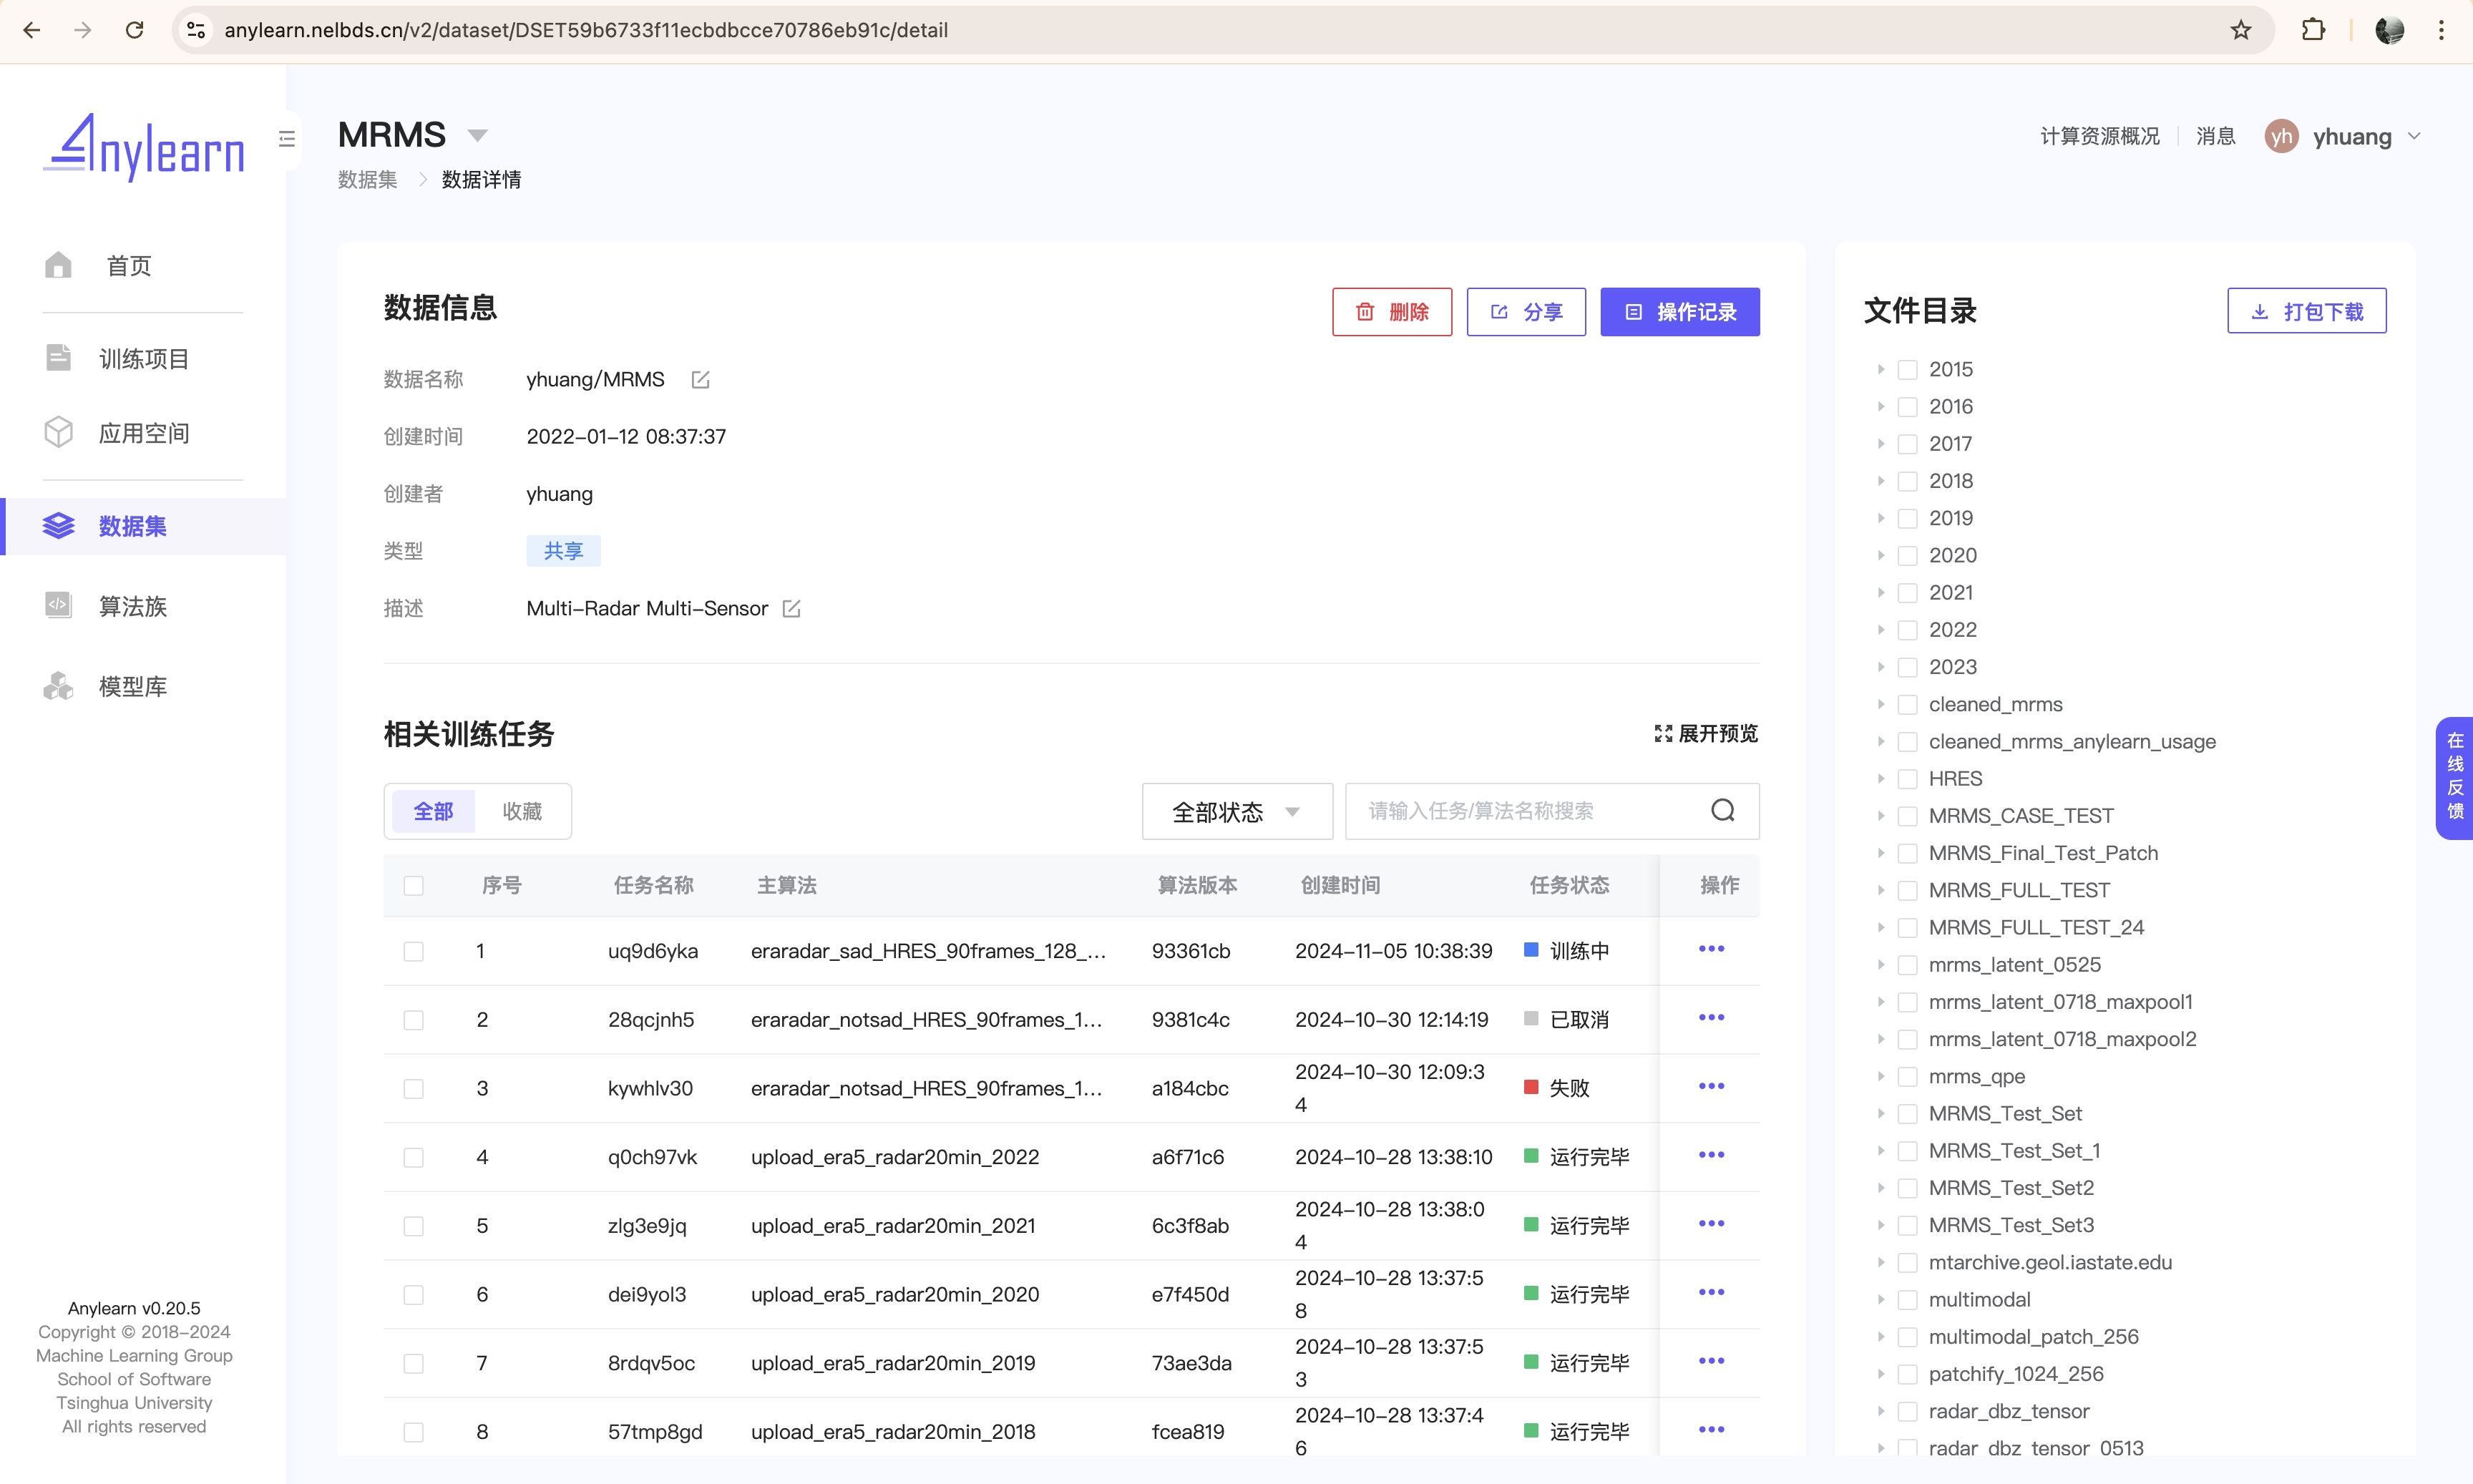
\includegraphics[width=0.98\linewidth]{mrms.jpg}
  \caption{Anylearn中的MRMS数据集}
  \label{fig:mrms}
\end{figure}

Anylearn的任务管理和资产管理可以有效地避免上述问题。
Anylearn底层的中心化文件存储可以保障数据处理、训练、验证等任务在不同节点执行时均可访问同一份数据集,无需在不同服务器上手动拷贝数据集。
负责数据处理工作的研发人员将数据处理脚本作为算法提交到Anylearn中进行管理和版本控制,确保数据处理方案不会遗失,同时也可以通过算法共享使团队内的其他研究人员了解数据处理过程的具体实现,促进沟通和讨论。
通过Anylearn数据处理任务在原始数据集上运行数据处理脚本并独立持久化存储处理后的数据,将脚本、原始数据集和处理后的数据集串联起来,满足后续的查询、检索、追溯等管理需求。
处理后的数据集可以作为数据处理任务结果共享给下游负责模型训练、验证、测试的研发人员,也可以写回原始数据集并共享给团队成员,满足团队协作需求。
所有雷达回波原始数据集以及处理后的数据集均通过Anylearn进行集约式的存储和管理,形成可追溯、可更新、可复用的数据集资产。
后续的模型训练、验证、测试等研发任务均以这些数据集资产为输入,能够以数据为中心地完整关联出模型研发过程中的各个阶段。

\subsection{模型开发迭代}
雷达回波外推模型研发的探索性强,需要基于不同的设计方案进行模型训练和效果验证,并不断迭代调整方案,在此过程中的实验记录格外重要。
由于缺乏便捷的实验记录工具,部分研发人员仍依赖电子表格手动记录实验,不仅效率低下,还容易遗漏重要数据。
人工记录的实验信息具有主观性,因人而异,在面临多人协作的使用场景时,需要人为制定记录规范才能较好地规避冲突,限制了沟通和讨论的效率。
此外,模型迭代的过程也是不断修改算法代码的过程,由此产生大量隐式的算法版本,很难通过人工记录的方式留存下每一次细微的代码变更并与训练结果形成关联,很容易导致方案的遗失。

使用了Anylearn,雷达回波外推模型研制过程中的上万次实验运行的元信息和实验方案代码均被自动化地记录了下来,确保每一次实验均可追溯的同时,省去了人工记录的工作量,避免了人工记录的谬误。
图\ref{fig:radartasks}展示了Anylearn中记录的雷达回波外推模型研发团队一位核心骨干成员的部分实验任务列表,最早的任务可追溯到2021年12月。
所有实验任务所使用的数据集、算法版本、超参数以及产生的结果等关键信息都被完整地持久化,便于研发人员溯源、交流、复盘。

\begin{figure}
  \centering
  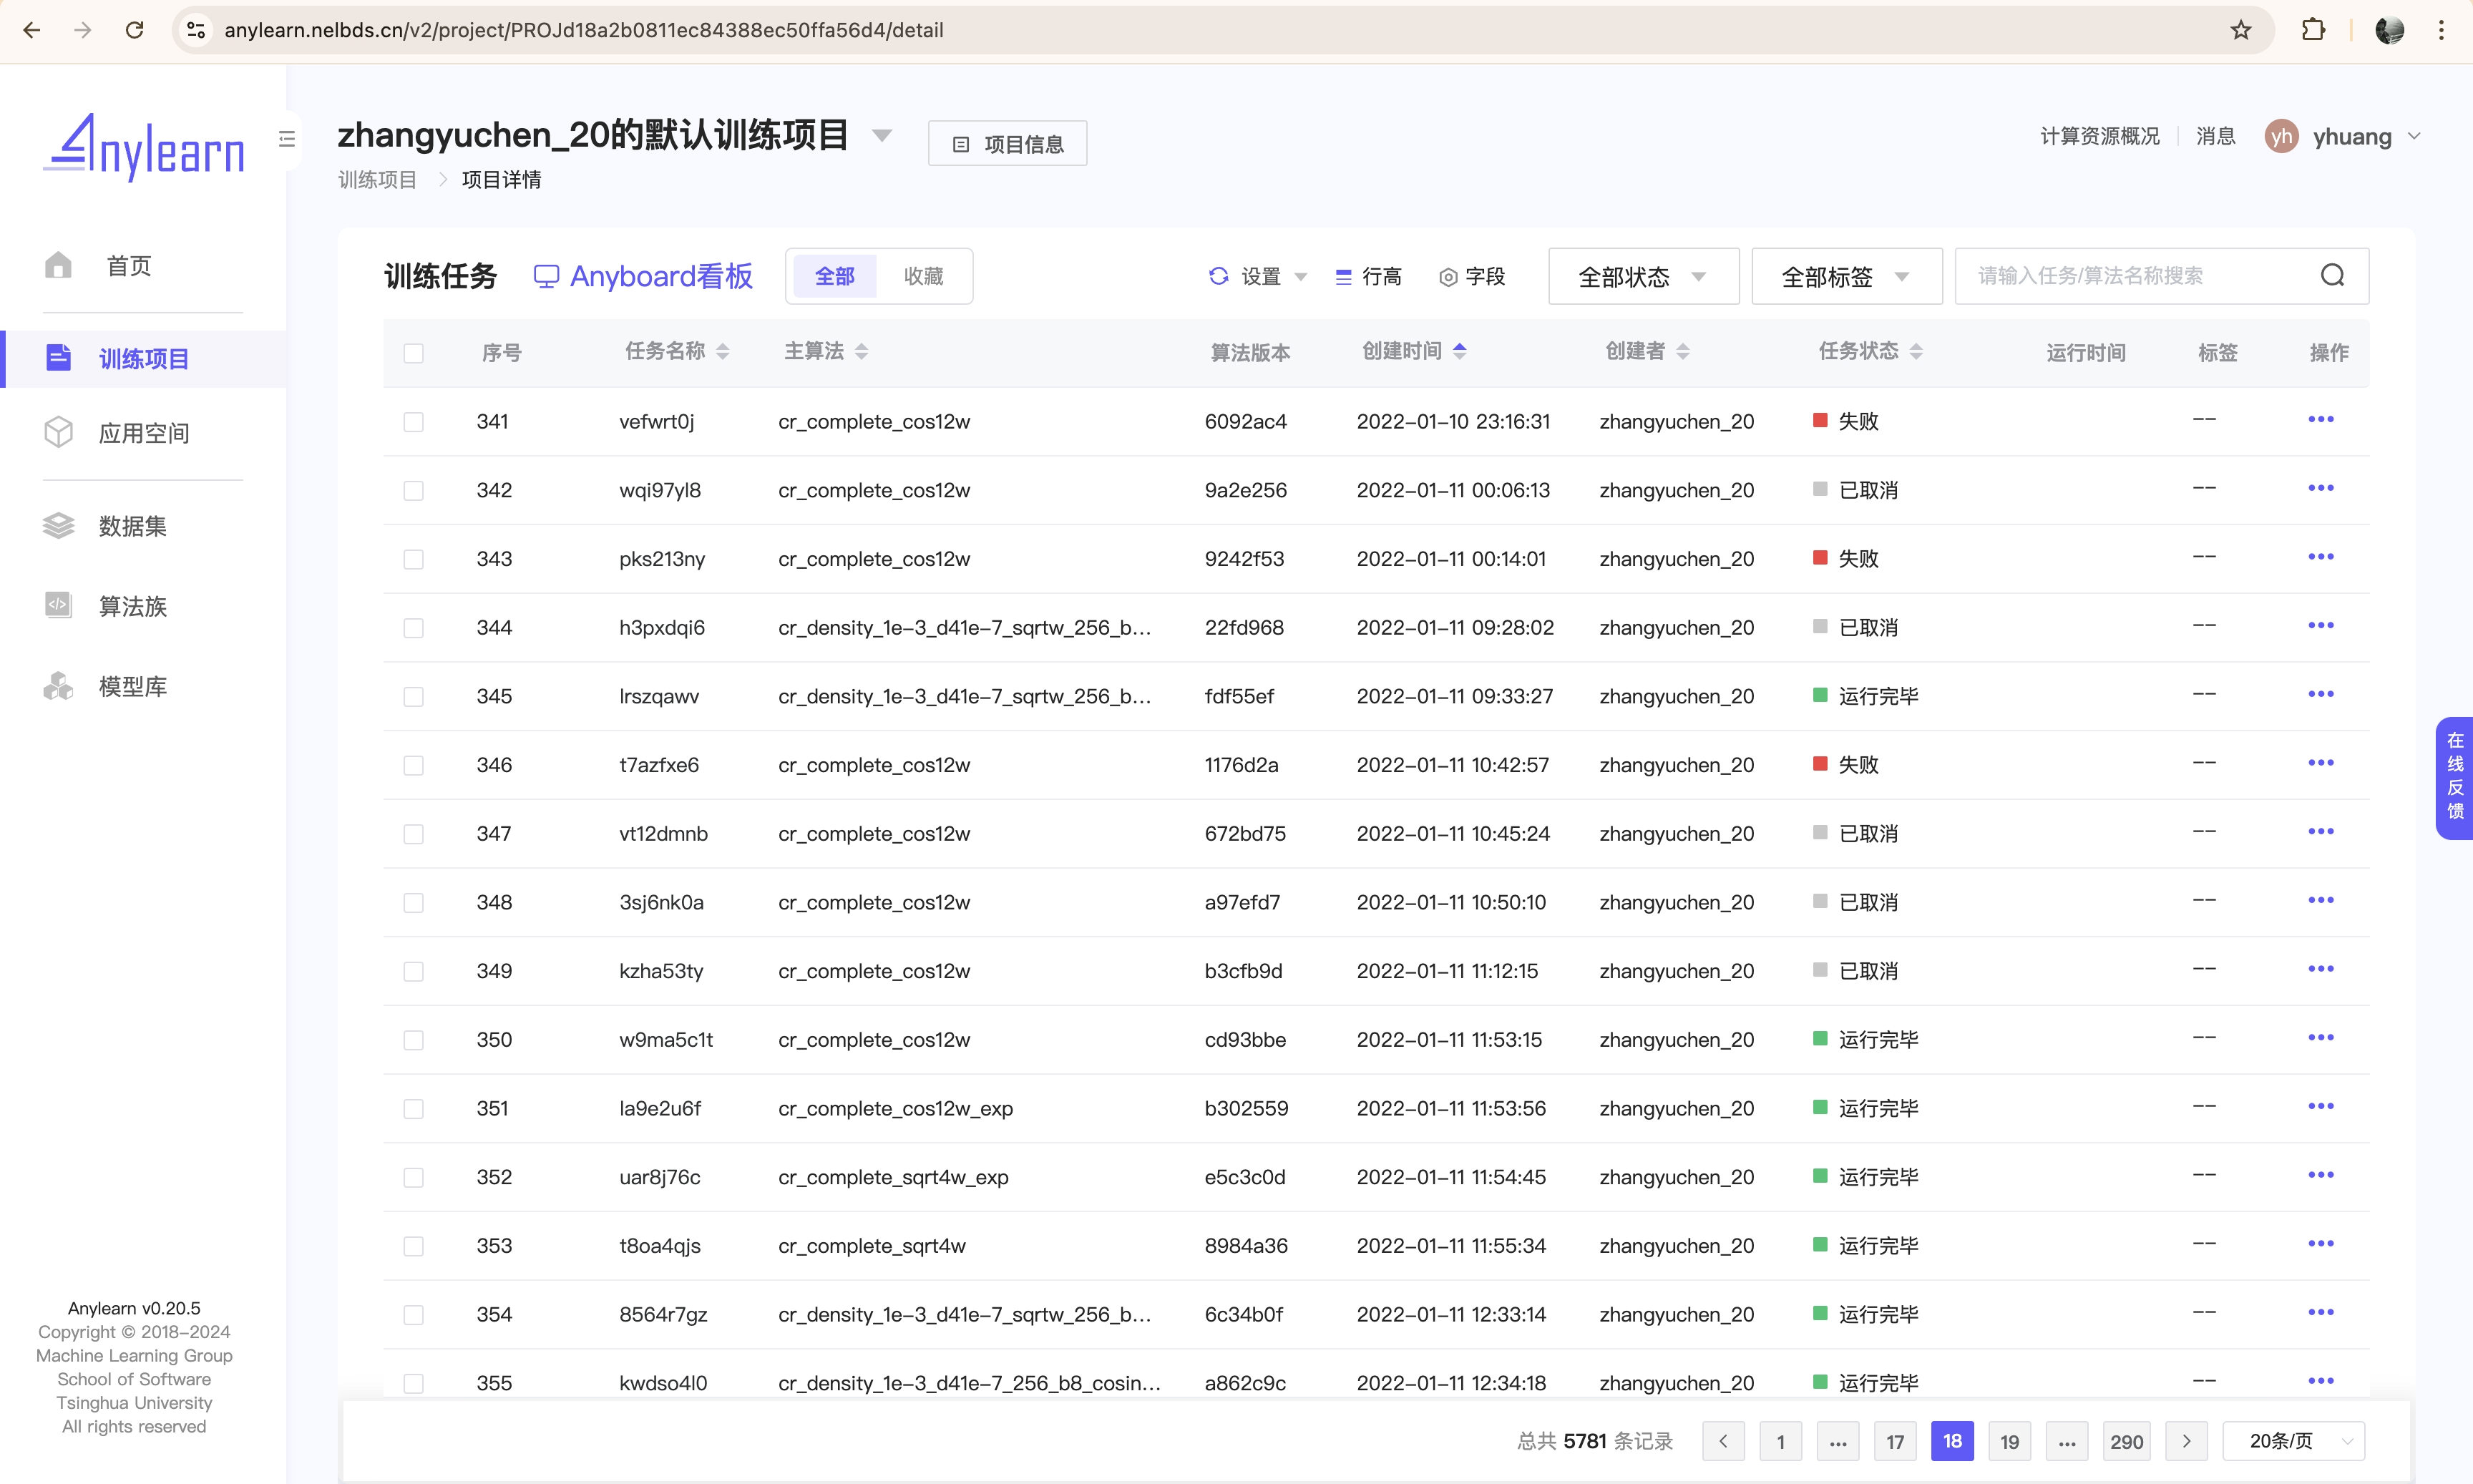
\includegraphics[width=0.98\linewidth]{radar-tasks.jpg}
  \caption{Anylearn中雷达回波外推模型研发相关的部分实验列表}
  \label{fig:radartasks}
\end{figure}

\subsection{模型效果预览}
目前学界和业界缺乏雷达回波外推的量化指标,对外推效果的评定往往依赖于肉眼观察雷达云图。
因此,在雷达回波外推模型的研发过程中,研究人员需要大量地生成模型预测出的雷达云图并评价其效果。

\begin{figure}
  \centering
  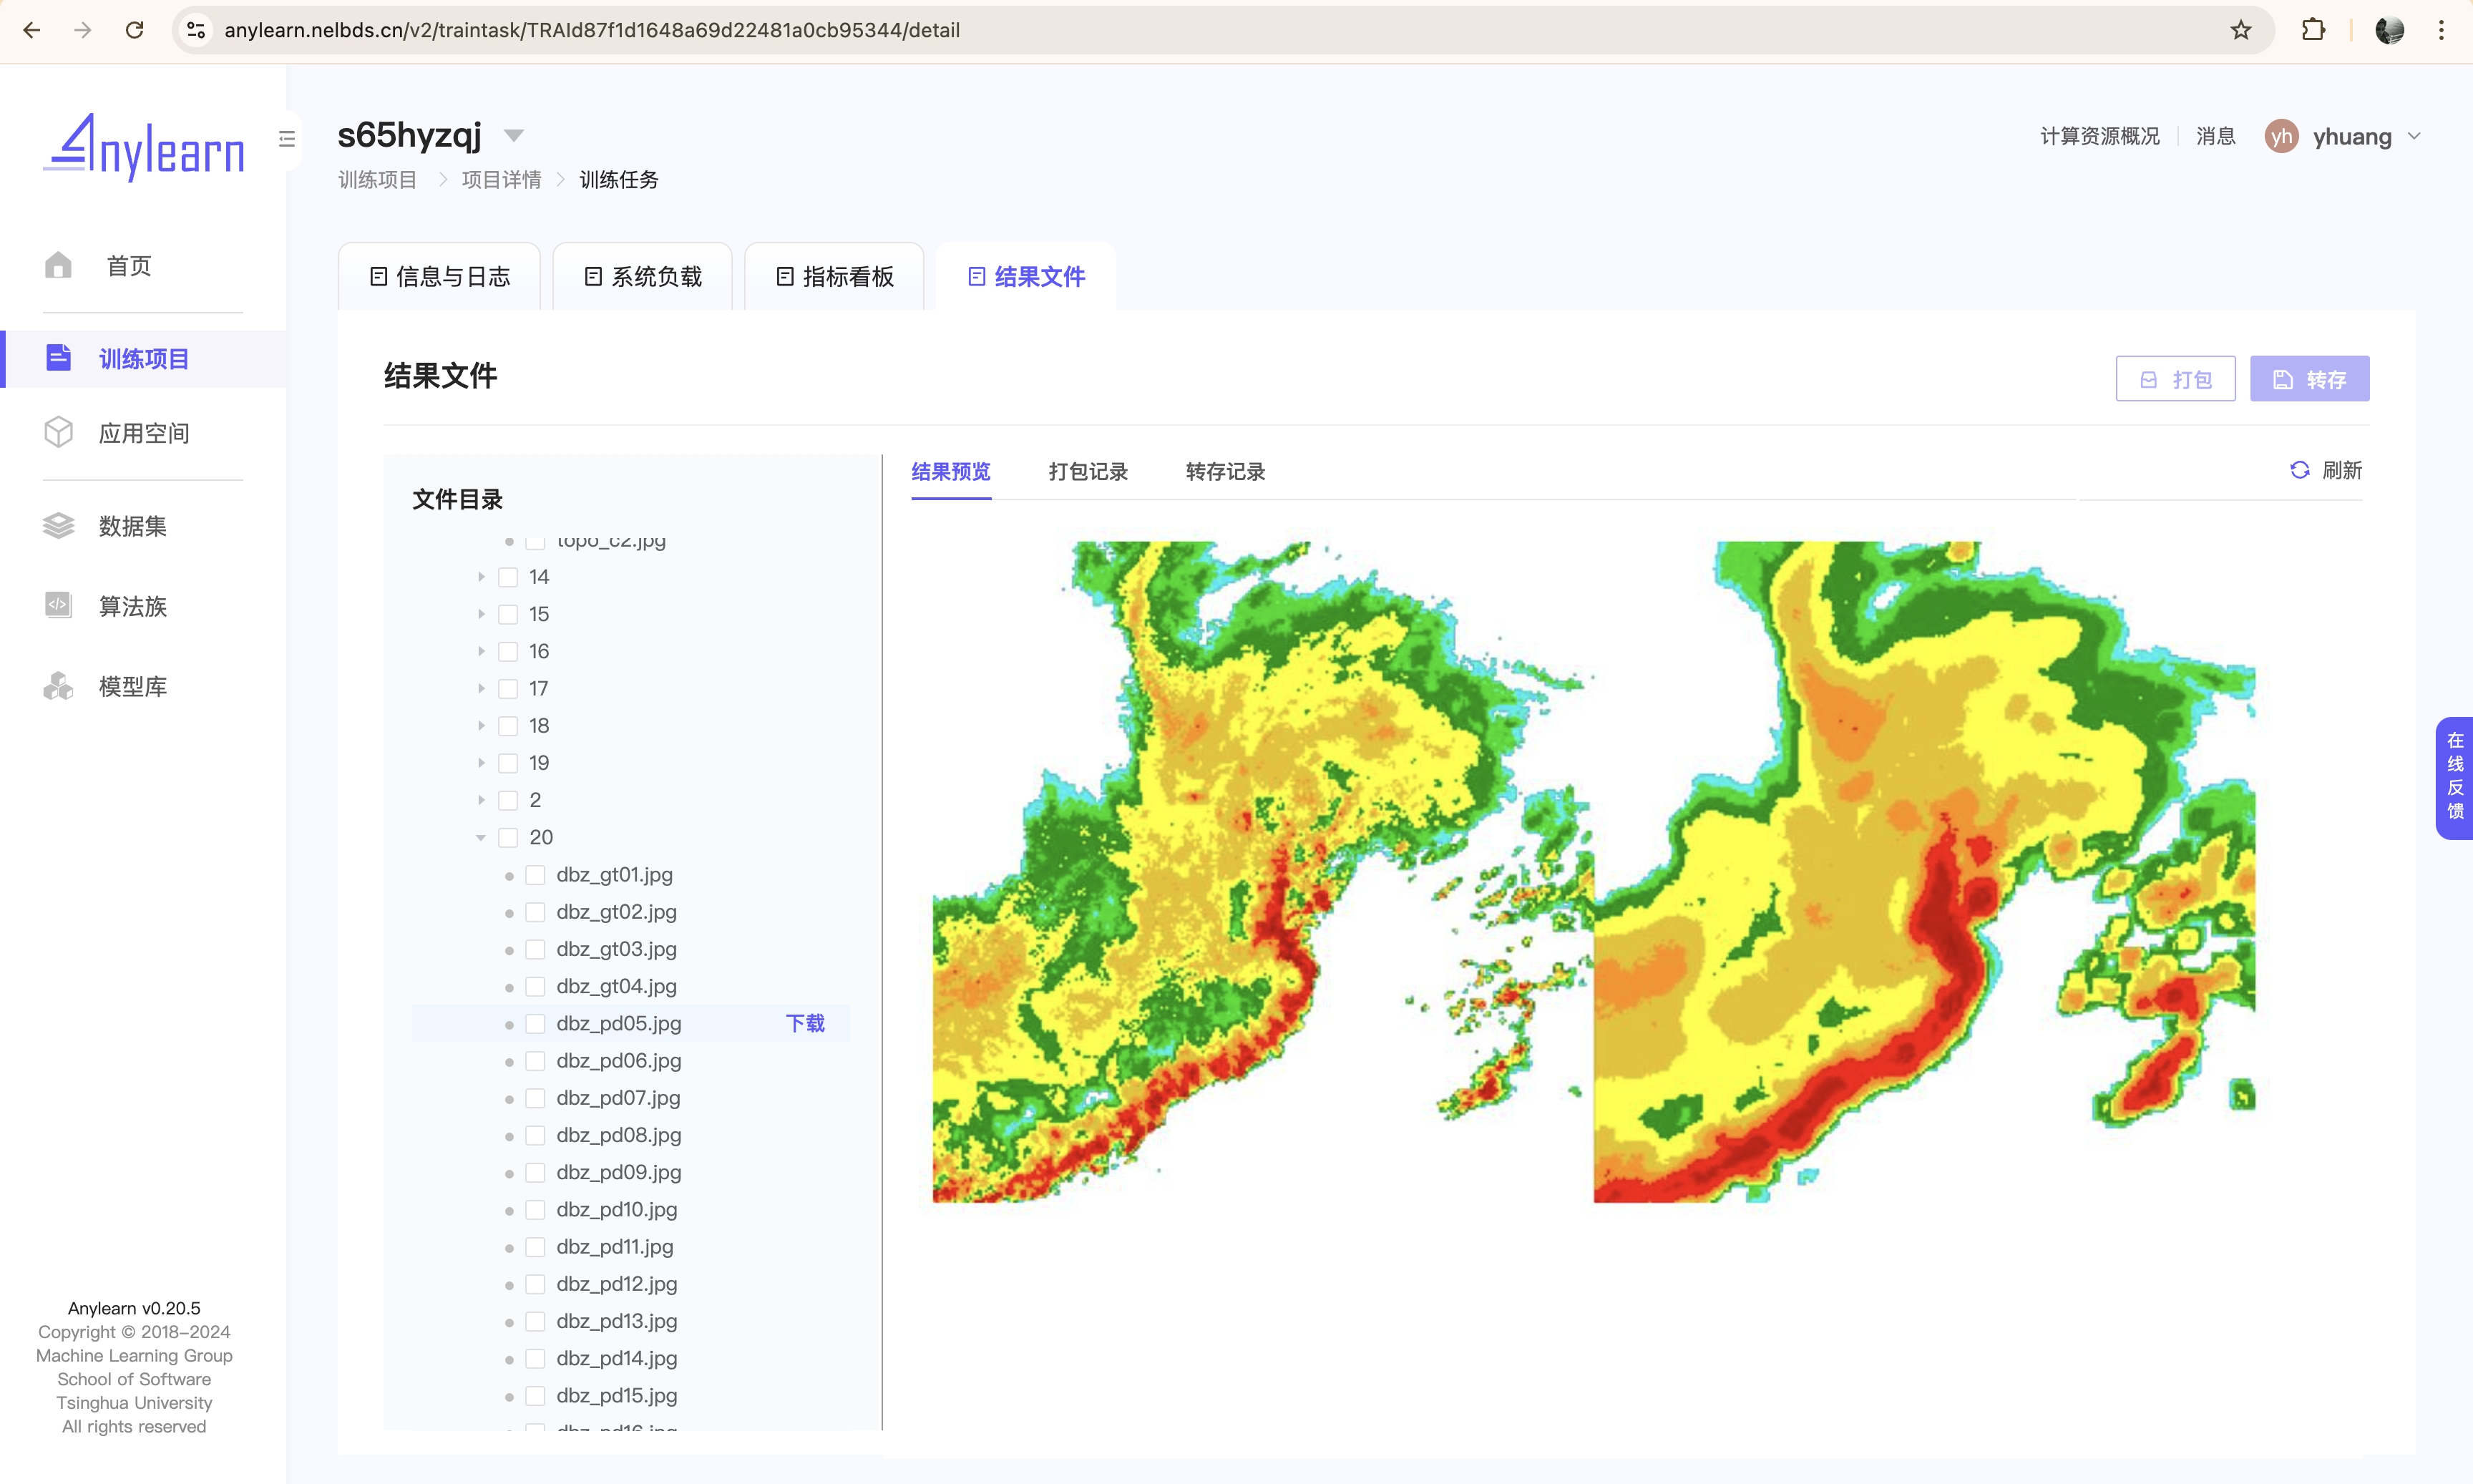
\includegraphics[width=0.98\linewidth]{radar-results.jpg}
  \caption{Anylearn中雷达回波外推实验结果可视化示例}
  \label{fig:radarresults}
\end{figure}

在未使用Anylearn之前,研究人员需要人工管理生成出的海量结果图片,并且经常需要将体积庞大的结果图包下载至个人电脑上进行查看。
而Anylearn能够自动地持久化每一次实验的结果文件,并原生支持在线查看图片类的结果文件,无需下载,完整覆盖了雷达回波外推模型评价的这一关键环节,如图\ref{fig:radarresults}所示。
此外,在雷达回波外推模型研发的后期需要专业气象预报专家在第三方系统中评测模型的效果,而Anylearn支持批量打包导出实验结果文件,有效地支撑了专家评测。
